\documentclass[border=10pt]{standalone}

\usepackage{tikz}
\usepackage{tikzsymbols}
\usetikzlibrary{calc,patterns,shapes.geometric}

\def\centerarc[#1](#2)(#3:#4:#5){\draw[#1] ($(#2)+({#5*cos(#3)},{#5*sin(#3)})$) arc (#3:#4:#5);}

\begin{document}
	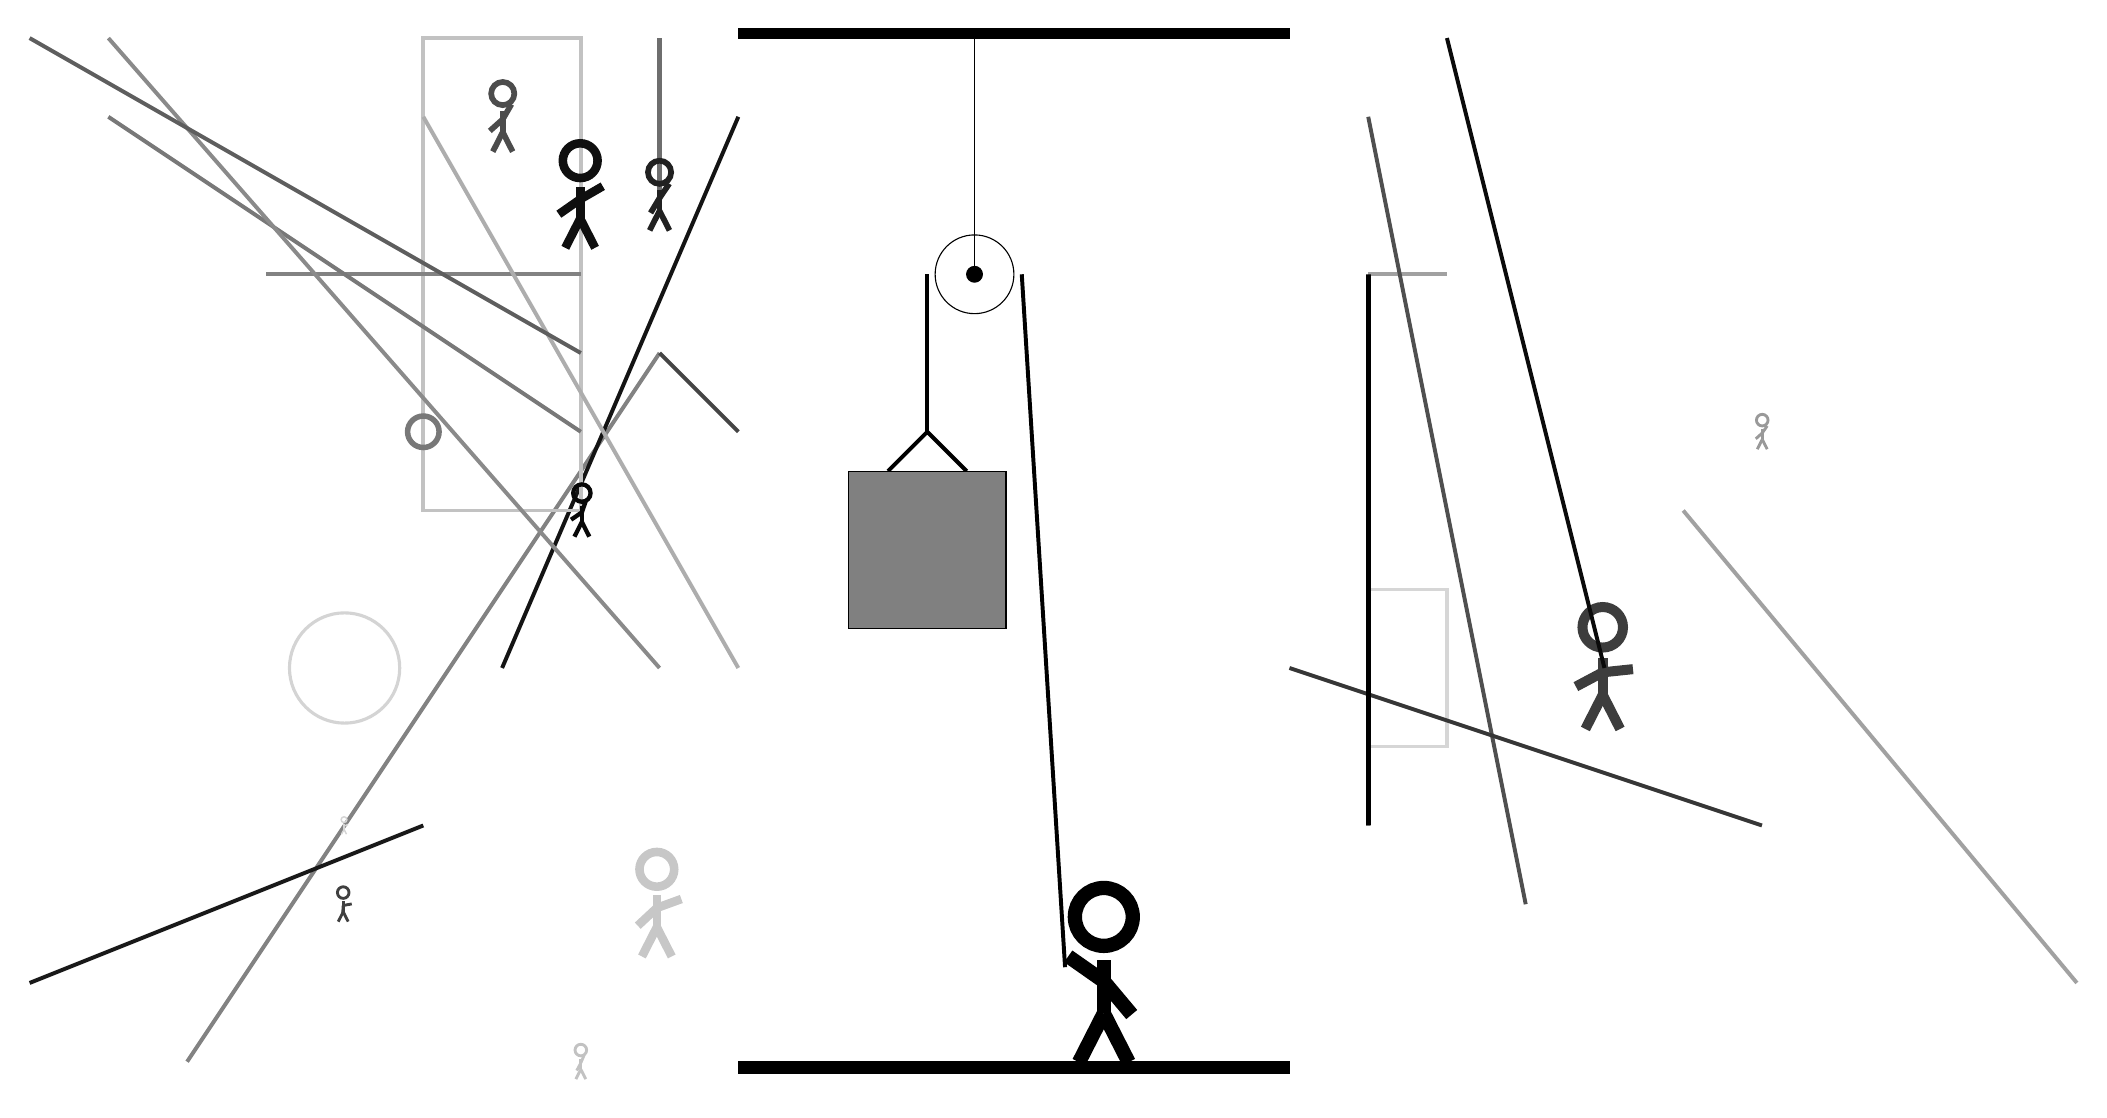
\begin{tikzpicture}
		%%%%% START %%%%%
		
		\draw[fill=black] (-2, 10) rectangle (5, 10.125);
		
		\draw (1, 7) circle (0.5);
		\draw[fill=black] (1, 7) circle (0.1);
		\draw (1, 10) -- (1, 7);
		
		\draw[line width=0.5mm] (-0.1, 4.5) -- (0.4, 5.0) -- (0.9, 4.5);
		\draw[fill=black!50] (-0.6, 4.5) rectangle (1.4, 2.5);
		
		\draw[line width=0.5mm] (0.4, 7) -- (0.4, 5.0);
		\centerarc[line width=0.5mm](1, 7)(0:180:0.6);
		\draw[line width=0.5mm](1.6, 7) -- (2.15, -1.8);
		
		\node at (2.6, -1.9) {\Strichmaxerl[10][-35][-50]};
		
		\draw[line width=0.5mm, color=black!94] (6, 0) rectangle (6, 1);
		
		\node[line width=0.3mm, color=black!75] at (-7, -1) {\Strichmaxerl[2][86][10]};
		\node[line width=0.5mm, color=black!24] at (-4, -3) {\Strichmaxerl[2][62][67]};
		\draw[line width=0.5mm, color=black!49](-3, 6) -- (-9, -3);
		\draw[line width=0.5mm, color=black!92](-5, 2) -- (-2, 9);
		\node[line width=0.6mm, color=black!40] at (11, 5) {\Strichmaxerl[2][42][55]};
		
		\draw[line width=0.5mm, color=black!24] (-4, 10) rectangle (-6, 4);
		\draw[line width=0.7mm, color=black!57] (-3, 8) rectangle (-3, 10);
		\node[line width=0.7mm, color=black!22] at (-3, -1) {\Strichmaxerl[6][43][20]};
		
		\draw[line width=0.5mm, color=black!73](-3, 6) -- (-2, 5);
		\node[line width=0.5mm, color=black!87] at (-3, 8) {\Strichmaxerl[4][59][56]};
		\node[line width=0.7mm, color=black!94] at (-4, 8) {\Strichmaxerl[6][35][30]};
		\node[line width=0.6mm, color=black!70] at (-5, 9) {\Strichmaxerl[4][42][60]};
		
		\draw[line width=0.5mm, color=black!49](-4, 7) -- (-8, 7);
		\draw [line width=0.3mm, color=black!17](9, 1) circle (0.0);
		\draw[line width=0.5mm, color=black!90](-6, 0) -- (-11, -2);
		
		\draw[line width=0.5mm, color=black!53](-4, 5) -- (-10, 9);
		\draw[line width=0.5mm, color=black!46](-3, 2) -- (-10, 10);
		\node[line width=0.4mm, color=black!17] at (-7, 0) {\Strichmaxerl[1][87][22]};
		\draw[line width=0.4mm, color=black!16] (6, 3) rectangle (7, 1);
		\node[line width=0.3mm, color=black!76] at (9, 2) {\Strichmaxerl[7][28][6]};
		
		\draw[line width=0.5mm, color=black!37] (6, 7) rectangle (7, 7);
		\draw [line width=0.3mm, color=black!39](5, 0) circle (0.0);
		\draw[line width=0.5mm, color=black!69](8, -1) -- (6, 9);
		\draw[line width=0.5mm, color=black!79](5, 2) -- (11, 0);
		
		\draw [line width=0.4mm, color=black!17](-7, 2) circle (0.7);
		\draw [line width=0.7mm, color=black!53](-6, 5) circle (0.2);
		\draw[line width=0.5mm, color=black!32](-2, 2) -- (-6, 9);
		\draw[line width=0.6mm, color=black!100] (6, 0) rectangle (6, 7);
		
		\draw[line width=0.5mm, color=black!96](9, 2) -- (7, 10);
		\draw[line width=0.5mm, color=black!37](10, 4) -- (15, -2);
		\draw[line width=0.5mm, color=black!63](-4, 6) -- (-11, 10);
		\node[line width=0.5mm, color=black!97] at (-4, 4) {\Strichmaxerl[3][34][71]};
		
		\draw[fill=black] (-2, -3) rectangle (5, -3.15);
		
		%%%%% END %%%%%
	\end{tikzpicture}
\end{document}